\begin{frame}{Première analyse du corpus Charcot}
\color{deepblue}{\textbf{OBVIE}\footnote{\url{https://obtic.huma-num.fr/obvie/}}}
\begin{itemize}
    \item moteur de recherche permettant la fouille avancée des corpus en \textsc{XML-TEI}
    \item identification des substantifs les plus importants 
    \begin{itemize}
        \item fréquences brutes, mesures \textsc{TF-IDF}, \textsc{BM25}, $\chi^2$, Test Gamma
    \end{itemize}
    \item repérage des textes similaires par ordre de pertinence
    \begin{itemize}
    \item à partir des termes en commun et termes fréquents
\end{itemize}     
\end{itemize}
    
\end{frame}
\begin{frame}{OBVIE -- corpus Charcot\footnote{\url{https://obtic.huma-num.fr/obvie/charcot/?view=corpus}}}
\danger{} impossible de quantifier l'importance des phrasèmes
\begin{figure}[!h]
    \centering
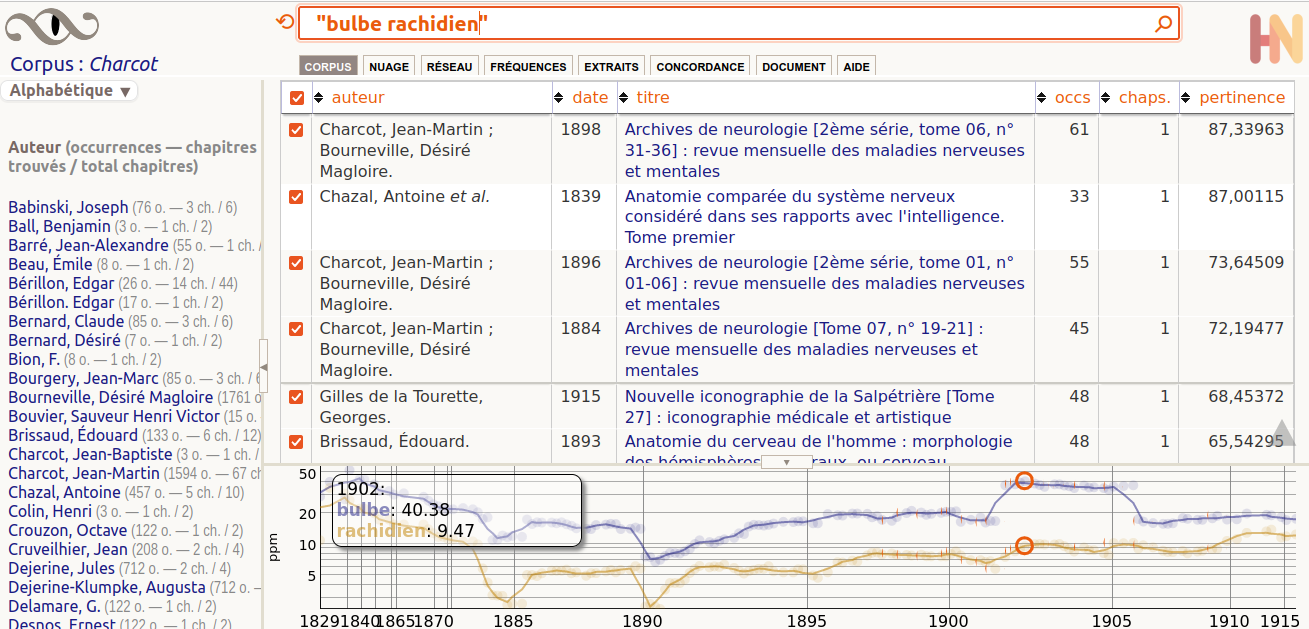
\includegraphics[width=90mm,scale=0.5]{pic/bulbe_rachidien.png}
    \caption{Distribution d'occurrences des tokens avec la frise chronologique pour ceux constituant l'expression \textit{bulbe rachidien}.}
    \label{fig:my_label}
\end{figure}
% citations directes (\cite{manjavacas2019})
\end{frame}

\begin{frame}{Deuxième analyse du corpus Charcot}
    \color{deepblue}{\textbf{TextPair}\footnote{\url{https://artfl-project.uchicago.edu/text-pair}}}
    \begin{itemize}
        \item aligne des passages similaires dans une collection de textes
        \begin{itemize}
        \item passages incluant des citations, plagiats, emprunts, réemplois$\dots$
        \end{itemize}
        \item génère une liste de séquences similaires pour chaque texte
        \begin{itemize}
        \item séquences de mots qui se chevauchent (trigrammes de mots)
        \end{itemize}        
        \item compare les séquences générées du texte \textit{source} au texte \textit{cible}
    \end{itemize}
\end{frame}

\begin{frame}{TextPair -- corpus Charcot\footnote{\url{https://anomander.uchicago.edu/text-pair/charcot2autres/}}}
\danger{} nombre de
résultats parfois assez conséquent $\rightarrow$ filtrage
    \begin{figure}[!ht]
        \centering
        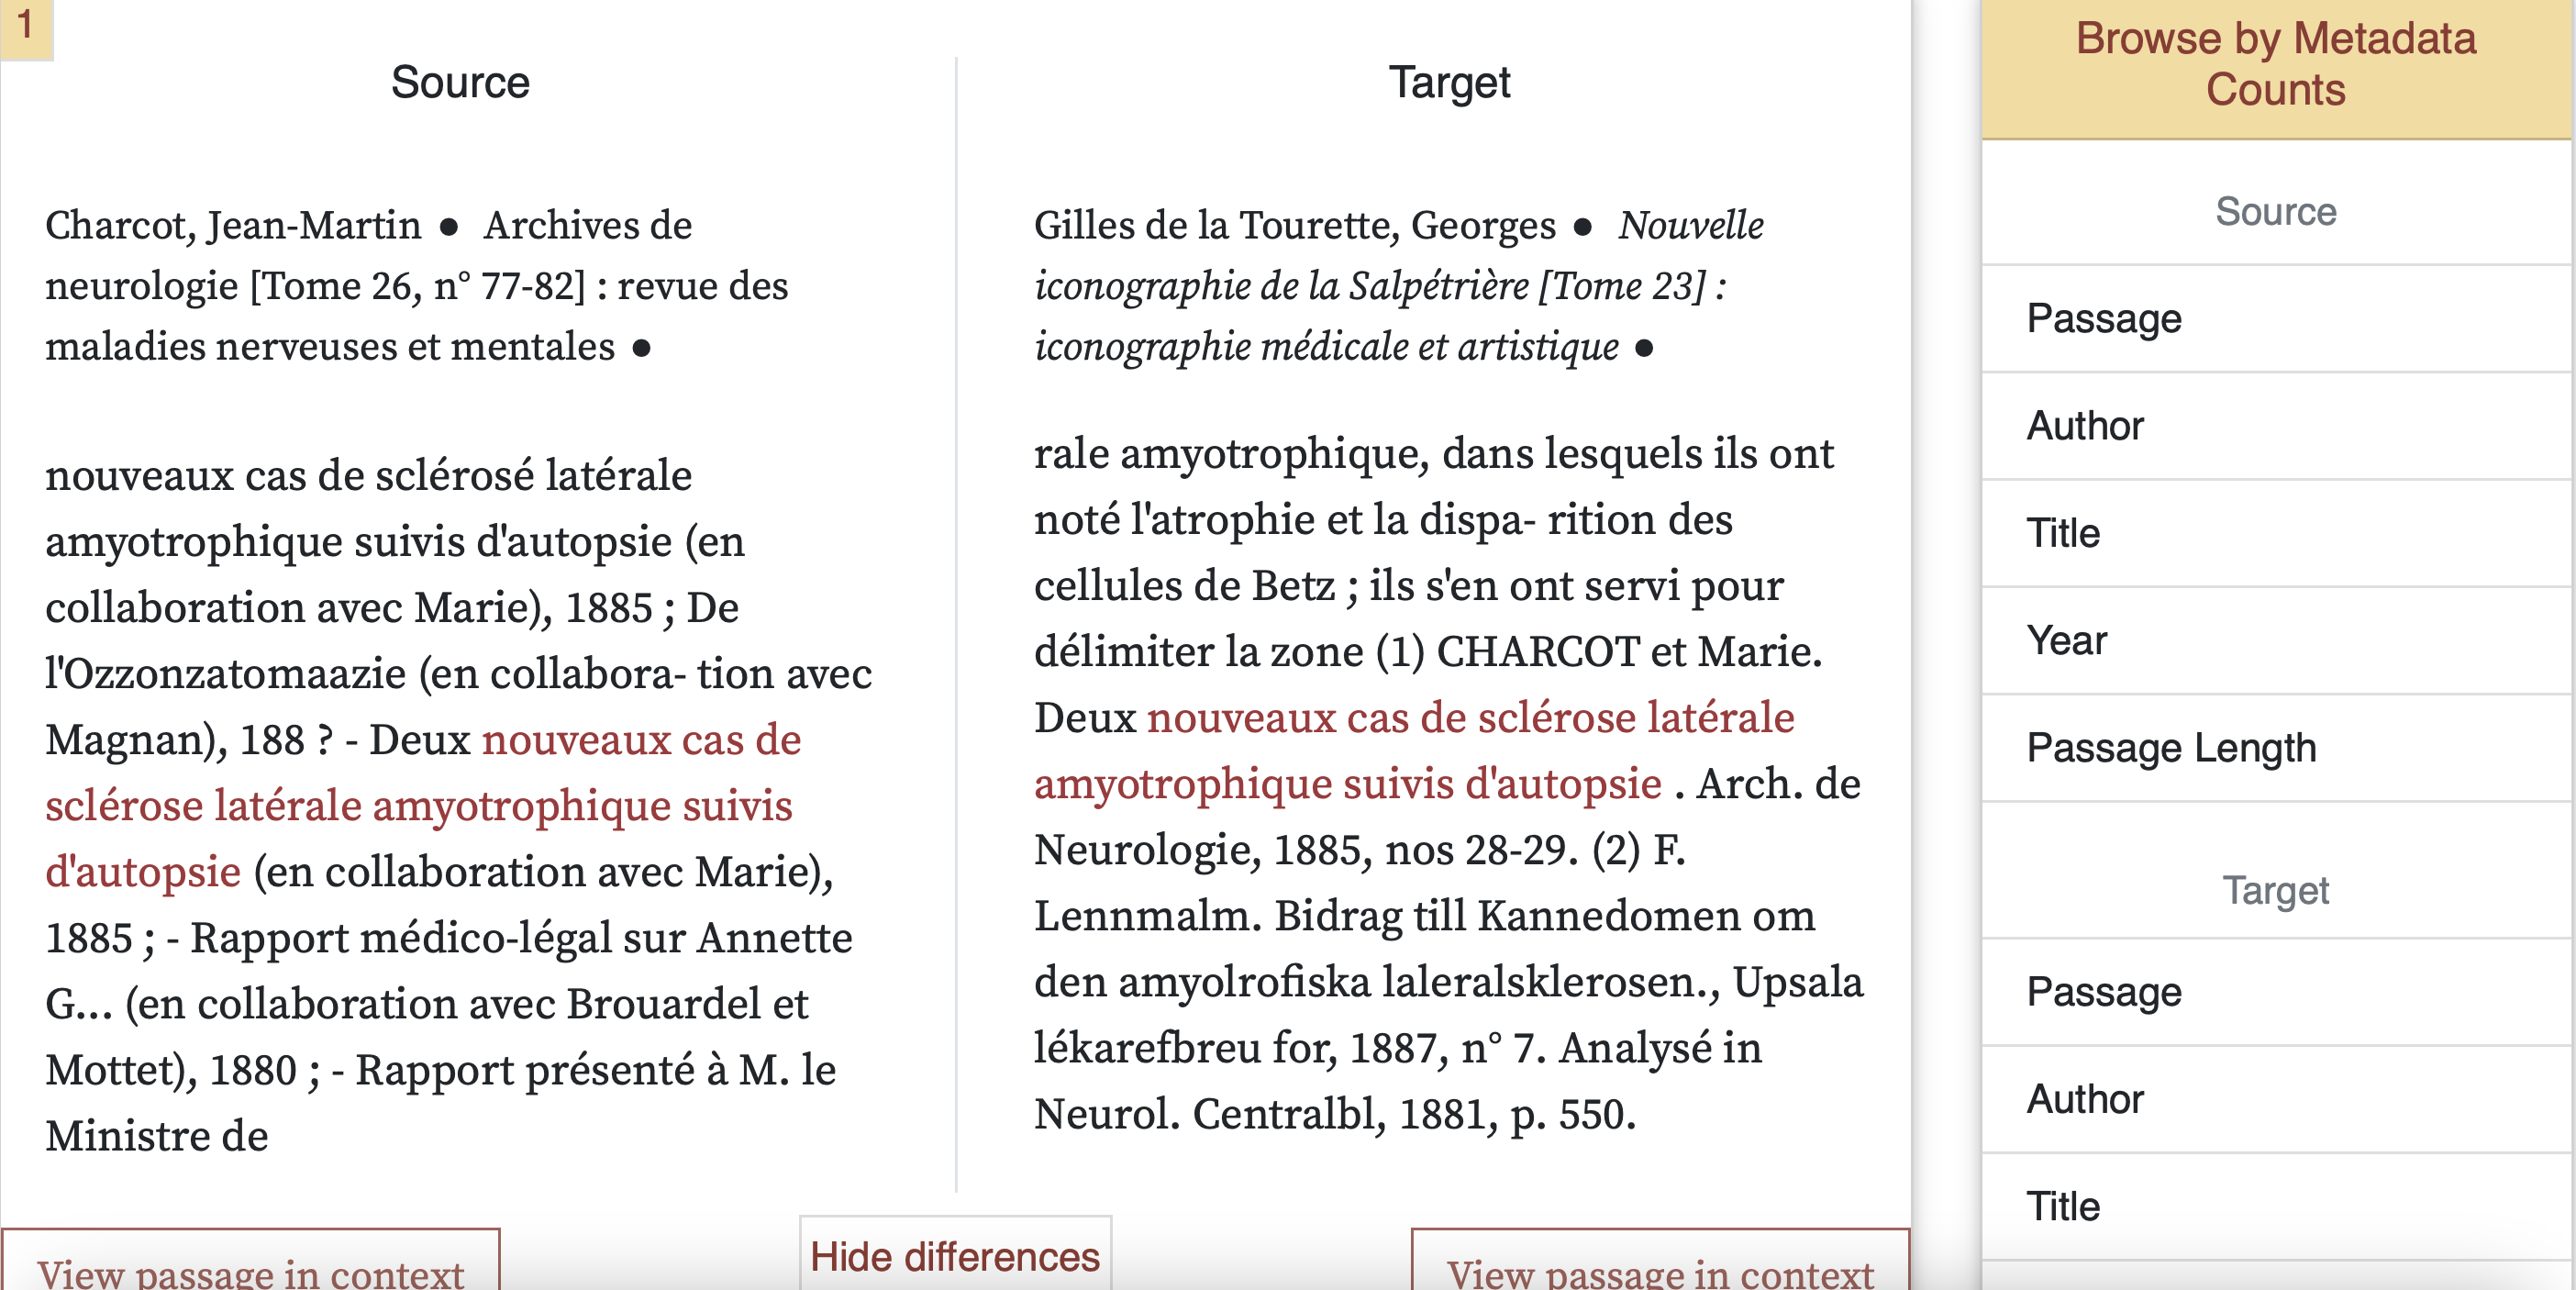
\includegraphics[width=90mm,scale=0.5]{pic/textpair.png}
        \caption{Réemploi du terme \textit{sclérose latérale amyotrophique} dans les textes de Charcot et de de la Tourette (le seul résultat).}
        \label{fig:enter-label}
    \end{figure}
\end{frame}
